The Standard Model (SM) of particle physics is a description of the physical world around us in terms of fundamental particles 
and their interactions. 
The development of the SM has been guided by both theoretical predictions and experimental discoveries.
The SM includes three of the four fundamental forces: electromagnetism, the strong interaction, and the weak interaction.
The mathematical formalism used relies on quantum field theory. %cite??

The fundamental particles are represented by the states of quantized fields.
Quarks and leptons constitute matter and are associated with fields of half integer spin, called fermion fields.
The dynamics of the system is defined by the Lagrangian, $\mathcal{L}$, a quantity that describes the motion and excitations 
in the fields.
The Lagrangian of the SM is invariant under spacetime dependent continuous internal transformations of the group 
$ SU\left(3\right) \times SU\left(2\right) \times U\left(1\right) $.
This invariance is called gauge invariance and is necessary to ensure that the theory is renormalizable.
The renormalizability condition guarantees the predictive power of the theory.
To preserve gauge invariance, additional quantum fields with spin one are required, called gauge bosons.
As a result, twelve gauge fields are required to write a gauge invariant Lagrangian, 
 eight for the generators of $ SU\left(3\right) $, three for the generators of $SU\left(2\right)$, 
and one for the $U\left(1\right)$ generator.
The elements described are enough to write down the Lagrangian of the SM.

\subsection{Quantum Chromodynamics}

The $ SU\left(3\right) $ gauge symmetry coupled to the quarks describes Quantum Chromodynamics (QCD), the theory of strong interactions.
The eight $ SU\left(3\right) $ gauge fields are associated to the different colored states of the gluon.
The QCD Lagrangian is given by
\begin{equation}
\mathcal{L}_{QCD} = -\frac{1}{4} G\indices{_{A\mu\nu}}G\indices{_{A}^{\mu\nu}} + \sum_{i=\text{flavors}} \overline{q}_i \left(i\slashed{D} - m_i\right) q_i,
\end{equation}
where $G$'s are the gauge fields of QCD given by 
\begin{equation}
G\indices{_{A\mu\nu}} = \partial_{\mu} G\indices{_{A\nu}} - \partial_{\nu} G\indices{_{A\mu}} - g_S f_{ABC} G\indices{_{B\mu}} G\indices{_{C\nu}},
\end{equation}
and the covariant derivative of QCD, $D\mu$,  defined as
\begin{equation}
D_\mu = \partial_{\mu} + i g_S \frac{\lambda_A}{2}G\indices{_{A\mu}},
\end{equation}
where $g_S$ is the strong coupling constant, and $\lambda_A$ are the eight Gell-Mann matrices.
The indices of the quarks, $i=1,2,3$, run over the colors: red, blue, green, and their anticolors.
While the indices of the gluons, $A,B,C = 1, \cdots, 8$, correspond to the combinations of colors and anticolors.
Color must be conserved in all QCD interactions, similar to the  electric charge.
Gluons have been inferred experimentally  and interact with quarks as predicted by the SM \cite{BRANDELIK1979243}.

\subsection{The Electroweak Theory}

The $ SU\left(2\right) \times U\left(1\right) $ gauge symmetry describes the
electroweak theory that unifies the electromagnetic and weak interactions.
There are two problems with this part of the SM.
The four gauge fields of $ SU\left(2\right) $ and $ U\left(1\right) $ 
must be added without mass to preserve gauge invariance.
However, the gauge bosons of the weak force have a large mass according to observation,
and thus in direct contradiction with the prediction.
%This problem was not relevant in the case of QCD since the gluons are massless. 
In addition, the weak interaction violates parity where it couples differently 
to the left and right-handed quark and lepton helicity states.
The solution is to treat the two helicity states of the leptons as different fields
with different couplings. A fermion mass term in the Lagrangian would couple to 
these different fields but will break gauge invariance.
Again to maintain gauge invariance, the fermion fields should be massless in 
direct contradiction with observation.

Both of the problems described can be resolved by introducing 
spontaneous symmetry breaking. The principle is to introduce new scalar fields with 
zero spin that couple to the electroweak  $ SU\left(2\right) \times U\left(1\right) $
gauge fields while preserving the gauge invariance of the Lagrangian.
The form of the potential describing this new interaction is chosen in such a way that 
zero values of the fields do not correspond to the lowest energy state.
As a consequence, the ground state of the field will ``break'' the  
$ SU\left(2\right) \times U\left(1\right) $ symmetry 
even though the Lagrangian preserves it.
The scalar fields will take a non-zero value, called the vacuum expectation value 
(vev), to allow the fermions and weak gauge bosons to appear as massive particles.
A consequence of this mechanism is that one additional scalar field obtains mass
and thus the theory predicts a neutral massive spin zero particle, the Higgs boson. 

The complete Lagrangian of the electroweak theory, including the mechanism 
of electroweak symmetry breaking, can then be expressed as
\begin{equation}
%\mathcal{L}_{EW} = \mathcal{L}_\text{gauge} + \mathcal{L}_\text{matter} +   \mathcal{L}_\text{Yukawa} + \mathcal{L}_\text{Higgs} .
\mathcal{L}_{EW} = \mathcal{L}_\text{gauge} + \mathcal{L}_\text{matter} + \mathcal{L}_\text{Higgs} +   \mathcal{L}_\text{Yukawa}  .
\end{equation}
The kinetic portion of the Lagrangian introduces the gauge isotriplet, $W\indices{_{\mu}^{i=1,2,3}}$, for 
 $ SU\left(2\right) $ and the gauge single, $B_\mu$, of $ U\left(1\right) $, in
\begin{equation}
\mathcal{L}_\text{gauge} =  -\frac{1}{4} \vect{W}\indices{_{\mu\nu}}\vect{W}\indices{^{\mu\nu}} - B\indices{_{\mu\nu}}B\indices{^{\mu\nu}},
\end{equation}
where 
\begin{equation}
\vect{W}^{\mu\nu} = \partial^{\mu}\vect{W}^{\nu} - \partial^{\nu} \vect{W}^{\mu} - g \vect{W}^{\mu} \times \vect{W}^{\nu},
\end{equation}
\begin{equation}
B\indices{^{\mu\nu}} = \partial^{\mu} B^{\nu} - \partial^{\nu} B^{\mu}
\end{equation}
and $g$ is the $ SU\left(2\right) $ gauge coupling constant. A linear superposition of the 
fields  $W\indices{_{\mu}^{i=1,2,3}}$ and $B_\mu$ lead to the SM $W^{\pm}$, $Z$, and photon.
The matter Lagrangian is
\begin{equation}
\mathcal{L}_\text{matter} = i\overline{\psi}\slashed{D}\psi
\end{equation}
where the covariant derivative of the electroweak theory is defined as
\begin{equation}
\label{eq:DmuEWK}
D_{\mu} = \partial_\mu + i g \vect{W}_\mu \cdot \vect{T} + \frac{1}{2}i g' B_{\mu}Y.
\end{equation}
where $g'$ is  $ U\left(1\right) $ gauge coupling constant, $\vect{T}$ is the weak isospin, and $Y$ is the weak hypercharge.
The Higgs potential introduces a doublet of complex scalar fields, $\Phi$, expressed as
\begin{equation}
 \mathcal{L}_\text{Higgs} = \left(D_\mu\Phi\right)^{\dagger} \left(D^\mu\Phi\right) + \mu^2 \Phi^{\dagger} \Phi - \lambda  \left(\Phi^{\dagger} \Phi \right)^2
\end{equation}
where $D_\mu$ is given in Eq. \ref{eq:DmuEWK} and 
\begin{equation}
\Phi = \left( \begin{matrix} \phi^+ \\ \phi^0\end{matrix} \right)
\end{equation}
The shape of the Higgs potential is determined by the parameters $\mu$ and $\lambda$. 
If $\mu^2 < 0$, the Higgs field will acquire a set of identical minima with a vev of 
$v=-\frac{\mu^2}{2\lambda} \equiv \frac{v^2}{2}$. The physical mass of the Higgs particle in the SM is
\begin{equation}
m_h = \sqrt{-2\mu^2},
\label{eq:theory.sm.mh}
\end{equation}
observed by ATLAS and CMS in 2012 with a mass of \\
$m_h = 125.09 \pm 0.24$ \GeV~\cite{atlas_higgs,cms_higgs}.
The Yukawa interactions are introduced to the Lagrangian manually to describe the interaction between the fermions and the Higgs field, 
expressed as 
\begin{equation}
 \mathcal{L}_\text{Yukawa} = \sum_\text{generations} \left[-\lambda_e \overline{L} \cdot \phi e_R - \lambda_d \overline{Q} \cdot \phi d_R 
 - \lambda_u \epsilon^{ab} \overline{Q}_a \phi_b^{\dagger} u_R + h.c. \right]
\end{equation}
where $\lambda$ is the Yukawa coupling of the particular fermion, $L$ and $e_R$ are the lepton fields, 
$Q$, $u_R$, and $d_R$ are the quark fields, $\epsilon^{ab} $ is the completely antisymmetric  $ SU\left(2\right) $ tensor 
with $\epsilon^{12} = 1$ ($\epsilon^{11} = \epsilon^{22} = 0$, $\epsilon^{21} = -1$).


\subsection{Limitations of the Standard Model}

The SM has now been tested successfully over the past decades which validated its dynamics in the gauge sector and in the flavor structure.
As an illustration of this remarkable achievement, Figure~\ref{fig:theory.sm.summary} shows the agreement between the SM total production cross section
of several processes that spans twelve orders of magnitude, 
measured by ATLAS compared to theoretical expectations 
at 7 \TeV, 8 \TeV, and 13 \TeV.
\begin{figure}[htb!]
\centering
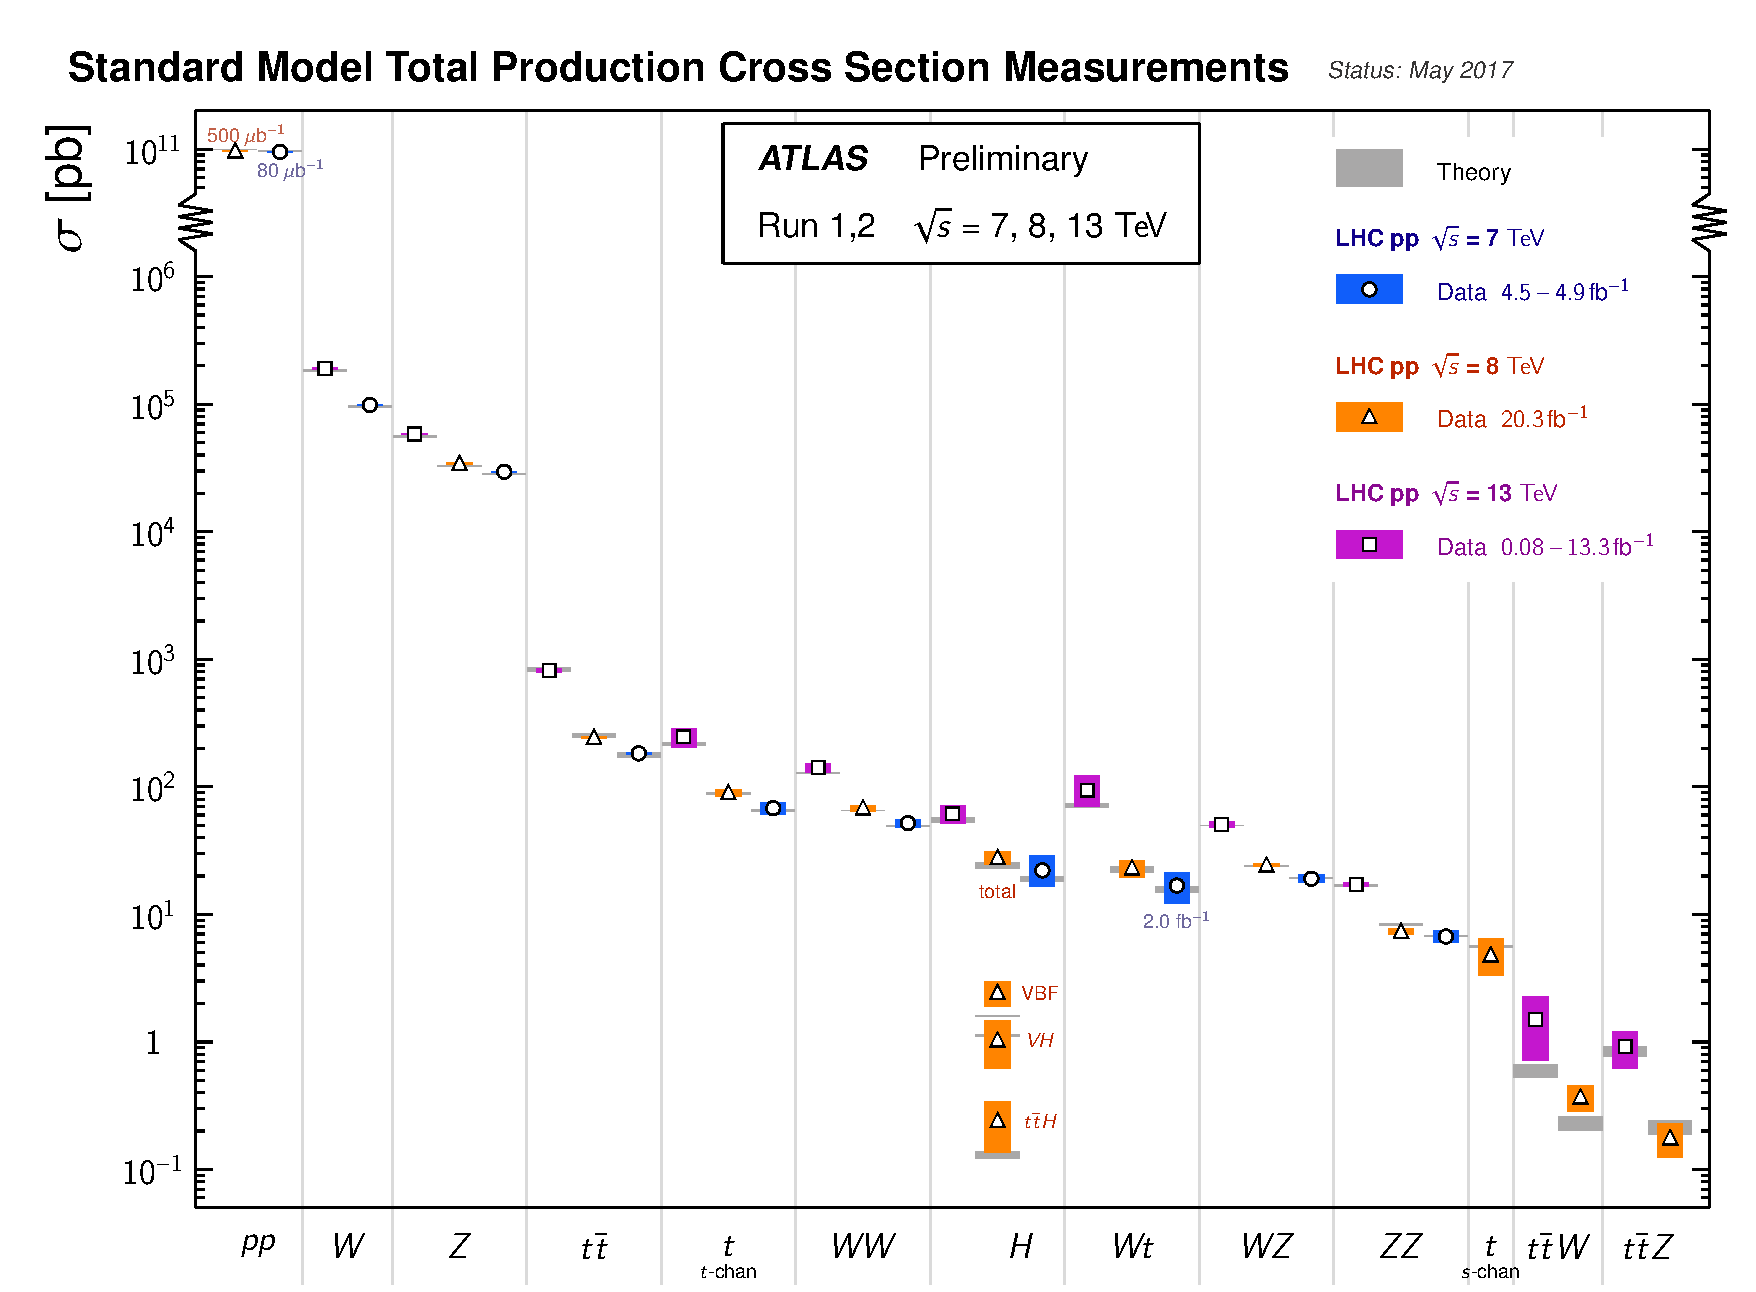
\includegraphics[width=0.95\textwidth]{atlas_sm_summary}
\caption{Summary of several Standard Model total production cross section measurements, corrected for leptonic branching fractions, 
compared to the corresponding theoretical expectations. All theoretical expectations were calculated at next-to-leading order or higher.}
\label{fig:theory.sm.summary}
\end{figure} 
The most obvious shortcoming is that the SM makes no attempt to include the fourth fundamental force of gravity. 
The reason is that the addition of the gravitational terms results in a theory that is not renormalizable, hence 
it looses its predictive power.
In the energy regime explored by modern accelerators, the impact of gravity is negligible. 
However, these effects become important at the Planck scale that corresponds to energies of 
$E_\text{Planck} = m_\text{Planck} c^2 = \sqrt{\hbar c^5/G_\text{Newton}} \sim 1.2 \times 10^{16}$ \TeV~(the LHC reaches $\sqrt{s}=13$ \TeV), 
which is well beyond our reach \cite{Ade:2013zuv}. 
Putting this problem aside, there are several problems in the energy range accessible to our accelerators:
\begin{itemize}
\item Dark matter: There is now overwhelming evidence for its existence; rotation curves, Cosmic Microwave Background, primordial abundance of the light elements, etc. 
Yet, the SM does not have a dark matter candidate\cite{Bertone:2004pz}.
\item Baryon asymmetry: The ratio of matter to antimatter is asymmetric with complete absence of antimatter except 
when temporarily formed, as in cosmic rays.
The asymmetry can be explained with the presence of $CP$-violating
\footnote{$CP$ refers to invariance under conjugation of (C) charge and (P) parity symmetries. 
The charge conjugation transforms a particle to its antiparticle while parity transforms the coordinate system to its mirror image.}
interactions. While the SM contains such $CP$ violating terms in the form of the Cabibbo–Kobayashi–Maskawa matrix, 
describing  quark mixing, and the Pontecorvo–Maki–Nakagawa–Sakata matrix, describing neutrino 
mixing, the size of this effect is too small to account for the observed asymmetry \cite{Canetti:2012zc}.
\item Anomalous magnetic moment of the muon: The measurement of the magnetic moment anomaly $a_\mu = \frac{g-2}{2}$, where $g$ is the gyromagnetic ratio of the muon, 
deviates from the SM prediction by 3.3$\sigma$ \cite{PhysRevD.73.072003,Hagiwara:2011af}.
\item Neutrino masses: The direct consequence of the observation of solar and atmospheric neutrino oscillations is that neutrinos are massive. The SM does not have a mechanism to include 
mass terms in its Lagrangian\cite{pdg}.
\end{itemize}
These arguments are not considered flaws of the SM but rather limitations that need to be overcome by adding new elements to the theory, i.e. new interactions and new particles.
None of the arguments mentioned address the question of the energy scale at which the new physics should appear.
For this, we turn to the two known scales in physics: the scale of electroweak physics of $\mathcal{O}\left(10^2\right)$ \GeV~and the scale of gravity of $\mathcal{O}\left(10^{19}\right)$ \GeV,
also known as the Planck scale.
The difference between the two scales is in the order of $\mathcal{O}\left(10^{16}\right)$. 
Since the SM is a renormalizable theory, it can be effectively valid up to the Planck scale and 
used to evaluate radiative corrections to any precision.
This causes a problem that can be best illustrated by calculating the mass of the Higgs boson in the SM.
The physical mass of the Higgs boson ( $m_\text{h,physical} \sim 125$ \GeV) can be written as $ m_\text{h,physical}^2 \simeq m_h^2 + \delta m_h^2$, 
where  $m_h$ is the Higgs mass parameter in the Lagrangian given in Eq. \ref{eq:theory.sm.mh}, and $\delta m_h$ is the one-loop radiative corrections 
obtained  by evaluating the diagrams of Figure~\ref{fig:theory.sm.oneloopH}.
\begin{figure}[htb!]
\centering
\begin{subfigure}[htb!]{0.32\textwidth}
\centering
\begin{fmffile}{sunset}
\begin{fmfgraph*}(75,75)
\fmfleft{i}
\fmfright{o}
\fmf{dashes,tension=5,label=$h$}{i,v1}
\fmf{dashes,tension=5,label=$h$}{v1,o}
\fmf{dashes,left,tension=0.75,label=$h$}{v1,v1}
\end{fmfgraph*}
\end{fmffile} 
\subcaption{}
\label{fig:}
\end{subfigure}
\begin{subfigure}[htb!]{0.32\textwidth}
\centering
\begin{fmffile}{sunset}
\begin{fmfgraph*}(75,75)
\fmfleft{i}
\fmfright{o}
\fmf{dashes,tension=5,label=$h$}{i,v1}
\fmf{dashes,tension=5,label=$h$}{v1,o}
\fmf{boson,left,tension=.75,label=$W,,Z$}{v1,v1}
\end{fmfgraph*}
\end{fmffile} 
\subcaption{}
\label{fig:}
\end{subfigure}
\begin{subfigure}[htb!]{0.32\textwidth}
\centering
\begin{fmffile}{sunset}
\begin{fmfgraph*}(75,75)
\fmfleft{i}
\fmfright{o}
\fmf{dashes,tension=5,label=$h$}{i,v1}
\fmf{dashes,tension=5,label=$h$}{v2,o}
\fmf{fermion,left,tension=1.5,label=$\ell,,q$}{v1,v2,v1}
\end{fmfgraph*}
\end{fmffile} 
\subcaption{}
\label{fig:}
\end{subfigure}
\vspace{-0.25cm}
\caption{The one-loop contribution of (a) quarks and leptons, (b) Higgs bosons, and (c) $W$,$Z$ bosons to the mass of the Higgs bosons.}
\label{fig:theory.sm.oneloopH}
\end{figure} 
The Higgs mass can then be expressed as
\begin{equation}
 m_\text{h,physical}^2 \simeq m_h^2 + \frac{C}{16\pi^2}\Lambda^2,
\end{equation}
where the coefficient $C$ embodies the various coupling constants of the SM\footnote{Expression can be found in equation (3) of \cite{Baer:2015fsa}.}.
The diagrams contributing to the Higgs mass diverge quadratically with $\Lambda$, the cut-off scale at which the SM is no longer valid.
If the diagrams do not mutually compensate for one another, the cut-off of quadratic divergences, $\Lambda$, can be as high as the Planck scale ($\mathcal{O}\left(10^{18}\right)$ \GeV).
In other words, the mass scale of the Higgs boson should be of the order of the Planck scale, while the observation is sixteen orders of magnitude below.
The mass parameter $m_h$ must be ``tuned'' to cancel out this huge correction.
This fine-tuning is regarded as \textit{unnatural} and a sign of undiscovered principles that would explain this hierarchy paradox, known as the ``hierarchy problem''.
By requiring that the quantum corrections, encoded in the cut-off scale $\Lambda$, should not be too far off from the mass parameter $m_h$, we can make an educated 
guess that the SM can only be valid up to an energy scale of $\Lambda \sim \mathcal{O}\left(1\right)$ \TeV~as illustrated in Figure~\ref{fig:theory.sm.deltamh2}.
\begin{figure}[htb!]
\centering
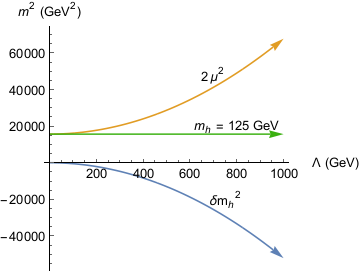
\includegraphics[width=0.75\textwidth]{deltamh2.png}
\caption{Illustration of how the Higgs mass parameter $m_h^2 = -2\mu^2$ needs to be adjusted to compensate for the quantum corrections $\delta m_h^2$ to ensure 
that $m_\text{h,physical} \sim 125$ \GeV~\cite{Bae:2015jea}.}
\label{fig:theory.sm.deltamh2}
\end{figure} 
This scale can be experimentally probed with the LHC to verify if new physics exists. Hence, the work presented in this dissertation is to search for new phenomena 
at this energy scale.
It is time to address the model studied in this dissertation that would resolve the hierarchy problem and some of the other limitations of the SM described in this section.
